\documentclass[a4paper]{book}
\usepackage{makeidx}
\usepackage{natbib}
\usepackage{graphicx}
\usepackage{multicol}
\usepackage{float}
\usepackage{listings}
\usepackage{color}
\usepackage{ifthen}
\usepackage[table]{xcolor}
\usepackage{textcomp}
\usepackage{alltt}
\usepackage{ifpdf}
\ifpdf
\usepackage[pdftex,
            pagebackref=true,
            colorlinks=true,
            linkcolor=blue,
            unicode
           ]{hyperref}
\else
\usepackage[ps2pdf,
            pagebackref=true,
            colorlinks=true,
            linkcolor=blue,
            unicode
           ]{hyperref}
\usepackage{pspicture}
\fi
\usepackage[utf8]{inputenc}
\usepackage{mathptmx}
\usepackage[scaled=.90]{helvet}
\usepackage{courier}
\usepackage{sectsty}
\usepackage[titles]{tocloft}
\usepackage{doxygen}
\lstset{language=C++,inputencoding=utf8,basicstyle=\footnotesize,breaklines=true,breakatwhitespace=true,tabsize=8,numbers=left }
\makeindex
\setcounter{tocdepth}{3}
\renewcommand{\footrulewidth}{0.4pt}
\renewcommand{\familydefault}{\sfdefault}
\hfuzz=15pt
\setlength{\emergencystretch}{15pt}
\hbadness=750
\tolerance=750
\begin{document}
\hypersetup{pageanchor=false,citecolor=blue}
\begin{titlepage}
\vspace*{7cm}
\begin{center}
{\Large gpio2440 }\\
\vspace*{1cm}
{\large \-Generated by Doxygen 1.7.6.1}\\
\vspace*{0.5cm}
{\small Mon Apr 1 2013 13:31:09}\\
\end{center}
\end{titlepage}
\clearemptydoublepage
\pagenumbering{roman}
\tableofcontents
\clearemptydoublepage
\pagenumbering{arabic}
\hypersetup{pageanchor=true,citecolor=blue}
\chapter{\-Class \-Index}
\section{\-Class \-Hierarchy}
\-This inheritance list is sorted roughly, but not completely, alphabetically\-:\begin{DoxyCompactList}
\item \contentsline{section}{gpiod\-\_\-ioc\-\_\-args}{\pageref{structgpiod__ioc__args}}{}
\item \contentsline{section}{\-Gpio\-Access\-:\-:\-Gpio\-Pin}{\pageref{class_gpio_access_1_1_gpio_pin}}{}
\begin{DoxyCompactList}
\item \contentsline{section}{\-Gpio\-Access\-:\-:\-Gpio\-Input\-Pin}{\pageref{class_gpio_access_1_1_gpio_input_pin}}{}
\item \contentsline{section}{\-Gpio\-Access\-:\-:\-Gpio\-Interrupt\-Pin$<$ \-T $>$}{\pageref{class_gpio_access_1_1_gpio_interrupt_pin}}{}
\item \contentsline{section}{\-Gpio\-Access\-:\-:\-Gpio\-Output\-Pin}{\pageref{class_gpio_access_1_1_gpio_output_pin}}{}
\end{DoxyCompactList}
\item \contentsline{section}{\-Gpio\-Access\-:\-:\-Gpio\-Port}{\pageref{class_gpio_access_1_1_gpio_port}}{}
\begin{DoxyCompactList}
\item \contentsline{section}{\-Gpio\-Access\-:\-:\-Gpio\-Input\-Port}{\pageref{class_gpio_access_1_1_gpio_input_port}}{}
\item \contentsline{section}{\-Gpio\-Access\-:\-:\-Gpio\-Output\-Port}{\pageref{class_gpio_access_1_1_gpio_output_port}}{}
\end{DoxyCompactList}
\item \contentsline{section}{\-Gpio\-Access\-:\-:\-Signal\-Action$<$ \-T $>$}{\pageref{struct_gpio_access_1_1_signal_action}}{}
\item \contentsline{section}{\-Test\-Class}{\pageref{class_test_class}}{}
\end{DoxyCompactList}

\chapter{\-Class \-Index}
\section{\-Class \-List}
\-Here are the classes, structs, unions and interfaces with brief descriptions\-:\begin{DoxyCompactList}
\item\contentsline{section}{\hyperlink{structgpiod__ioc__args}{gpiod\-\_\-ioc\-\_\-args} }{\pageref{structgpiod__ioc__args}}{}
\item\contentsline{section}{\hyperlink{class_gpio_access_1_1_gpio_input_pin}{\-Gpio\-Access\-::\-Gpio\-Input\-Pin} }{\pageref{class_gpio_access_1_1_gpio_input_pin}}{}
\item\contentsline{section}{\hyperlink{class_gpio_access_1_1_gpio_input_port}{\-Gpio\-Access\-::\-Gpio\-Input\-Port} }{\pageref{class_gpio_access_1_1_gpio_input_port}}{}
\item\contentsline{section}{\hyperlink{class_gpio_access_1_1_gpio_interrupt_pin}{\-Gpio\-Access\-::\-Gpio\-Interrupt\-Pin$<$ T $>$} }{\pageref{class_gpio_access_1_1_gpio_interrupt_pin}}{}
\item\contentsline{section}{\hyperlink{class_gpio_access_1_1_gpio_output_pin}{\-Gpio\-Access\-::\-Gpio\-Output\-Pin} }{\pageref{class_gpio_access_1_1_gpio_output_pin}}{}
\item\contentsline{section}{\hyperlink{class_gpio_access_1_1_gpio_output_port}{\-Gpio\-Access\-::\-Gpio\-Output\-Port} }{\pageref{class_gpio_access_1_1_gpio_output_port}}{}
\item\contentsline{section}{\hyperlink{class_gpio_access_1_1_gpio_pin}{\-Gpio\-Access\-::\-Gpio\-Pin} }{\pageref{class_gpio_access_1_1_gpio_pin}}{}
\item\contentsline{section}{\hyperlink{class_gpio_access_1_1_gpio_port}{\-Gpio\-Access\-::\-Gpio\-Port} }{\pageref{class_gpio_access_1_1_gpio_port}}{}
\item\contentsline{section}{\hyperlink{struct_gpio_access_1_1_signal_action}{\-Gpio\-Access\-::\-Signal\-Action$<$ T $>$} }{\pageref{struct_gpio_access_1_1_signal_action}}{}
\item\contentsline{section}{\hyperlink{class_test_class}{\-Test\-Class} }{\pageref{class_test_class}}{}
\end{DoxyCompactList}

\chapter{\-Class \-Documentation}
\hypertarget{structgpiod__ioc__args}{\section{gpiod\-\_\-ioc\-\_\-args \-Struct \-Reference}
\label{structgpiod__ioc__args}\index{gpiod\-\_\-ioc\-\_\-args@{gpiod\-\_\-ioc\-\_\-args}}
}
\subsection*{\-Public \-Attributes}
\begin{DoxyCompactItemize}
\item 
\hypertarget{structgpiod__ioc__args_a20ea304329455b464a0e12ca1caa237b}{int {\bfseries pid}}\label{structgpiod__ioc__args_a20ea304329455b464a0e12ca1caa237b}

\item 
\hypertarget{structgpiod__ioc__args_afdbbb73a282759c017e318e20e0cdfe4}{unsigned int {\bfseries pin}}\label{structgpiod__ioc__args_afdbbb73a282759c017e318e20e0cdfe4}

\item 
\hypertarget{structgpiod__ioc__args_a2cc2eb135fea1cbeef461f0908aa2225}{unsigned int {\bfseries value}}\label{structgpiod__ioc__args_a2cc2eb135fea1cbeef461f0908aa2225}

\end{DoxyCompactItemize}


\subsection{\-Detailed \-Description}


\-Definition at line 4 of file gpio2440.\-h.



\-The documentation for this struct was generated from the following file\-:\begin{DoxyCompactItemize}
\item 
src/driver/gpio2440.\-h\end{DoxyCompactItemize}

\hypertarget{class_gpio_access_1_1_gpio_input_pin}{\section{\-Gpio\-Access\-:\-:\-Gpio\-Input\-Pin \-Class \-Reference}
\label{class_gpio_access_1_1_gpio_input_pin}\index{\-Gpio\-Access\-::\-Gpio\-Input\-Pin@{\-Gpio\-Access\-::\-Gpio\-Input\-Pin}}
}


{\ttfamily \#include $<$\-Gpio\-Input\-Pin.\-h$>$}

\-Inheritance diagram for \-Gpio\-Access\-:\-:\-Gpio\-Input\-Pin\-:\begin{figure}[H]
\begin{center}
\leavevmode
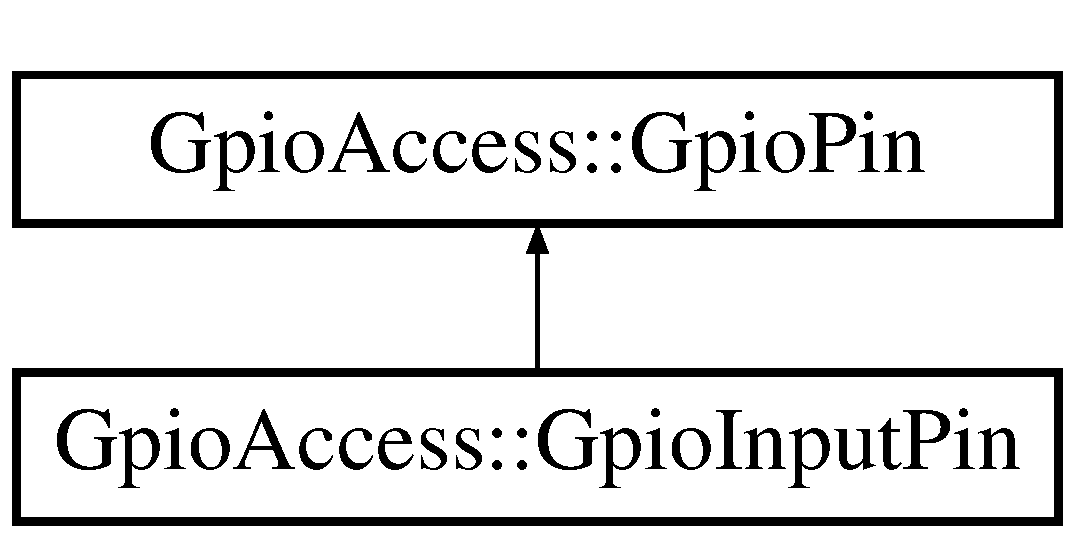
\includegraphics[height=2.000000cm]{class_gpio_access_1_1_gpio_input_pin}
\end{center}
\end{figure}
\subsection*{\-Public \-Member \-Functions}
\begin{DoxyCompactItemize}
\item 
\hyperlink{class_gpio_access_1_1_gpio_input_pin_a32dbeb898419c64462d4f136bea92221}{\-Gpio\-Input\-Pin} (int \hyperlink{class_gpio_access_1_1_gpio_pin_a662d9f6e22d338e0b182b3220a42f25d}{gpio\-Id}=0, bool pull\-Up=true)
\end{DoxyCompactItemize}


\subsection{\-Detailed \-Description}
\hyperlink{class_gpio_access_1_1_gpio_input_pin}{\-Gpio\-Input\-Pin} es la clase que define las funcionalidades de un puerto de entrada. 

\-Definition at line 16 of file \-Gpio\-Input\-Pin.\-h.



\subsection{\-Constructor \& \-Destructor \-Documentation}
\hypertarget{class_gpio_access_1_1_gpio_input_pin_a32dbeb898419c64462d4f136bea92221}{\index{\-Gpio\-Access\-::\-Gpio\-Input\-Pin@{\-Gpio\-Access\-::\-Gpio\-Input\-Pin}!\-Gpio\-Input\-Pin@{\-Gpio\-Input\-Pin}}
\index{\-Gpio\-Input\-Pin@{\-Gpio\-Input\-Pin}!GpioAccess::GpioInputPin@{\-Gpio\-Access\-::\-Gpio\-Input\-Pin}}
\subsubsection[{\-Gpio\-Input\-Pin}]{\setlength{\rightskip}{0pt plus 5cm}{\bf \-Gpio\-Access\-::\-Gpio\-Input\-Pin\-::\-Gpio\-Input\-Pin} (
\begin{DoxyParamCaption}
\item[{int}]{gpio\-Id = {\ttfamily 0}, }
\item[{bool}]{pull\-Up = {\ttfamily true}}
\end{DoxyParamCaption}
)}}\label{class_gpio_access_1_1_gpio_input_pin_a32dbeb898419c64462d4f136bea92221}
\-Constructor de \hyperlink{class_gpio_access_1_1_gpio_input_pin}{\-Gpio\-Input\-Pin}. 
\begin{DoxyParams}{\-Parameters}
{\em p\-Gpio\-Id} & es un entero que contiene el identificador del puerto a utilizar. \\
\hline
{\em pull\-Up} & alor booleano que define la configuracion del resistor pullup. \\
\hline
\end{DoxyParams}

\begin{DoxyExceptions}{\-Exceptions}
{\em runtime\-\_\-error.} & \\
\hline
\end{DoxyExceptions}


\-Definition at line 10 of file \-Gpio\-Input\-Pin.\-cpp.



\-The documentation for this class was generated from the following files\-:\begin{DoxyCompactItemize}
\item 
src/access/\-Gpio\-Input\-Pin.\-h\item 
src/access/\-Gpio\-Input\-Pin.\-cpp\end{DoxyCompactItemize}

\hypertarget{class_gpio_access_1_1_gpio_input_port}{\section{\-Gpio\-Access\-:\-:\-Gpio\-Input\-Port \-Class \-Reference}
\label{class_gpio_access_1_1_gpio_input_port}\index{\-Gpio\-Access\-::\-Gpio\-Input\-Port@{\-Gpio\-Access\-::\-Gpio\-Input\-Port}}
}


{\ttfamily \#include $<$\-Gpio\-Input\-Port.\-h$>$}

\-Inheritance diagram for \-Gpio\-Access\-:\-:\-Gpio\-Input\-Port\-:\begin{figure}[H]
\begin{center}
\leavevmode
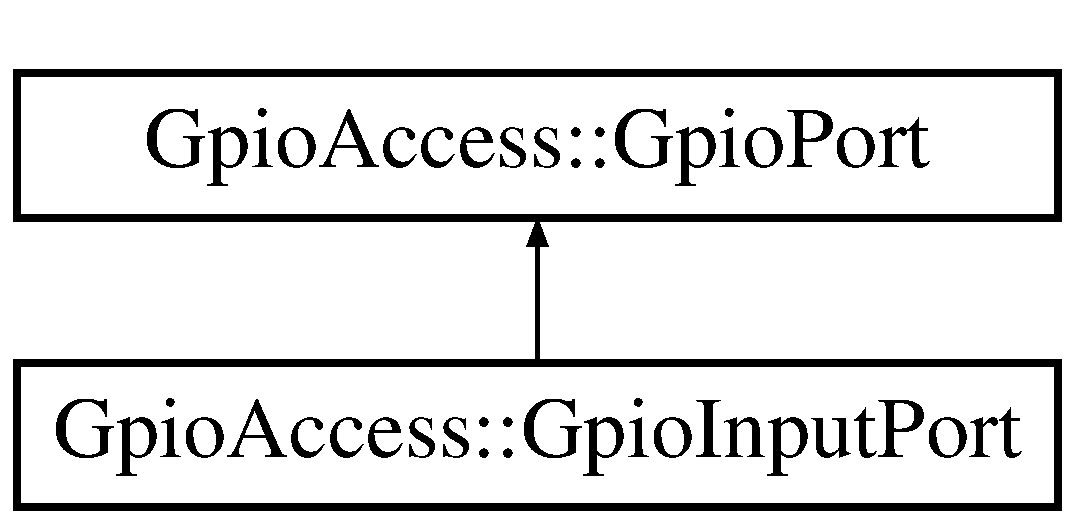
\includegraphics[height=2.000000cm]{class_gpio_access_1_1_gpio_input_port}
\end{center}
\end{figure}
\subsection*{\-Public \-Member \-Functions}
\begin{DoxyCompactItemize}
\item 
\hyperlink{class_gpio_access_1_1_gpio_input_port_aeeed64420582ca1ebc2d741e140b67b9}{\-Gpio\-Input\-Port} (int $\ast$bits\-Ids, int \hyperlink{class_gpio_access_1_1_gpio_port_a7708b465b3c98a32e592ee985c3dcf8b}{bit\-Count}, bool pull\-Up=true)
\item 
unsigned int \hyperlink{class_gpio_access_1_1_gpio_input_port_aeed5b1a3eccb39dd6cff6f2e281a890b}{read} ()
\item 
\hypertarget{class_gpio_access_1_1_gpio_input_port_abda439bc45285d6cac9776ab8b61a978}{bool {\bfseries operator\mbox{[}$\,$\mbox{]}} (unsigned int pos)}\label{class_gpio_access_1_1_gpio_input_port_abda439bc45285d6cac9776ab8b61a978}

\end{DoxyCompactItemize}
\subsection*{\-Protected \-Attributes}
\begin{DoxyCompactItemize}
\item 
\hyperlink{class_gpio_access_1_1_gpio_input_pin}{\-Gpio\-Access\-::\-Gpio\-Input\-Pin} $\ast$ \hyperlink{class_gpio_access_1_1_gpio_input_port_a4817dfd3065aebdb9d9231f54bff8ba5}{input\-Bits}
\end{DoxyCompactItemize}


\subsection{\-Detailed \-Description}
\hyperlink{class_gpio_access_1_1_gpio_input_port}{\-Gpio\-Input\-Port} es la clase que define las funcionalidades de un bus de entrada. 

\-Definition at line 21 of file \-Gpio\-Input\-Port.\-h.



\subsection{\-Constructor \& \-Destructor \-Documentation}
\hypertarget{class_gpio_access_1_1_gpio_input_port_aeeed64420582ca1ebc2d741e140b67b9}{\index{\-Gpio\-Access\-::\-Gpio\-Input\-Port@{\-Gpio\-Access\-::\-Gpio\-Input\-Port}!\-Gpio\-Input\-Port@{\-Gpio\-Input\-Port}}
\index{\-Gpio\-Input\-Port@{\-Gpio\-Input\-Port}!GpioAccess::GpioInputPort@{\-Gpio\-Access\-::\-Gpio\-Input\-Port}}
\subsubsection[{\-Gpio\-Input\-Port}]{\setlength{\rightskip}{0pt plus 5cm}{\bf \-Gpio\-Access\-::\-Gpio\-Input\-Port\-::\-Gpio\-Input\-Port} (
\begin{DoxyParamCaption}
\item[{int $\ast$}]{bits\-Ids, }
\item[{int}]{bit\-Count, }
\item[{bool}]{pull\-Up = {\ttfamily true}}
\end{DoxyParamCaption}
)}}\label{class_gpio_access_1_1_gpio_input_port_aeeed64420582ca1ebc2d741e140b67b9}
\-Constructor de \hyperlink{class_gpio_access_1_1_gpio_input_port}{\-Gpio\-Input\-Port}. 
\begin{DoxyParams}{\-Parameters}
{\em bits\-Ids} & es un arreglo de enteros los cuales corresponden con los identificadores de los puertos que conforman el bus de entrada. \\
\hline
{\em p\-Bit\-Count} & cantidad de bits del bus de entrada. \\
\hline
{\em pull\-Up} & valor booleano que define la configuracion del resistor pullup. \\
\hline
\end{DoxyParams}


\-Definition at line 8 of file \-Gpio\-Input\-Port.\-cpp.



\subsection{\-Member \-Function \-Documentation}
\hypertarget{class_gpio_access_1_1_gpio_input_port_aeed5b1a3eccb39dd6cff6f2e281a890b}{\index{\-Gpio\-Access\-::\-Gpio\-Input\-Port@{\-Gpio\-Access\-::\-Gpio\-Input\-Port}!read@{read}}
\index{read@{read}!GpioAccess::GpioInputPort@{\-Gpio\-Access\-::\-Gpio\-Input\-Port}}
\subsubsection[{read}]{\setlength{\rightskip}{0pt plus 5cm}unsigned int {\bf \-Gpio\-Access\-::\-Gpio\-Input\-Port\-::read} (
\begin{DoxyParamCaption}
{}
\end{DoxyParamCaption}
)}}\label{class_gpio_access_1_1_gpio_input_port_aeed5b1a3eccb39dd6cff6f2e281a890b}
\-La función read lee el valor presente en el bus. \begin{DoxyReturn}{\-Returns}
\-Devuelve un valor entero positivo correspondiente a la lectura del bus de entrada. 
\end{DoxyReturn}

\begin{DoxyExceptions}{\-Exceptions}
{\em runtime\-\_\-error.} & \\
\hline
\end{DoxyExceptions}


\-Definition at line 20 of file \-Gpio\-Input\-Port.\-cpp.



\subsection{\-Member \-Data \-Documentation}
\hypertarget{class_gpio_access_1_1_gpio_input_port_a4817dfd3065aebdb9d9231f54bff8ba5}{\index{\-Gpio\-Access\-::\-Gpio\-Input\-Port@{\-Gpio\-Access\-::\-Gpio\-Input\-Port}!input\-Bits@{input\-Bits}}
\index{input\-Bits@{input\-Bits}!GpioAccess::GpioInputPort@{\-Gpio\-Access\-::\-Gpio\-Input\-Port}}
\subsubsection[{input\-Bits}]{\setlength{\rightskip}{0pt plus 5cm}{\bf \-Gpio\-Access\-::\-Gpio\-Input\-Pin}$\ast$ {\bf \-Gpio\-Access\-::\-Gpio\-Input\-Port\-::input\-Bits}\hspace{0.3cm}{\ttfamily  \mbox{[}protected\mbox{]}}}}\label{class_gpio_access_1_1_gpio_input_port_a4817dfd3065aebdb9d9231f54bff8ba5}
input\-Bits es un arreglo donde se almacenan los puertos que componen el bus de entrada. 

\-Definition at line 50 of file \-Gpio\-Input\-Port.\-h.



\-The documentation for this class was generated from the following files\-:\begin{DoxyCompactItemize}
\item 
src/access/\-Gpio\-Input\-Port.\-h\item 
src/access/\-Gpio\-Input\-Port.\-cpp\end{DoxyCompactItemize}

\hypertarget{class_gpio_access_1_1_gpio_interrupt_pin}{\section{\-Gpio\-Access\-:\-:\-Gpio\-Interrupt\-Pin$<$ \-T $>$ \-Class \-Template \-Reference}
\label{class_gpio_access_1_1_gpio_interrupt_pin}\index{\-Gpio\-Access\-::\-Gpio\-Interrupt\-Pin$<$ T $>$@{\-Gpio\-Access\-::\-Gpio\-Interrupt\-Pin$<$ T $>$}}
}


{\ttfamily \#include $<$\-Gpio\-Interrupt\-Pin.\-h$>$}

\-Inheritance diagram for \-Gpio\-Access\-:\-:\-Gpio\-Interrupt\-Pin$<$ \-T $>$\-:\begin{figure}[H]
\begin{center}
\leavevmode
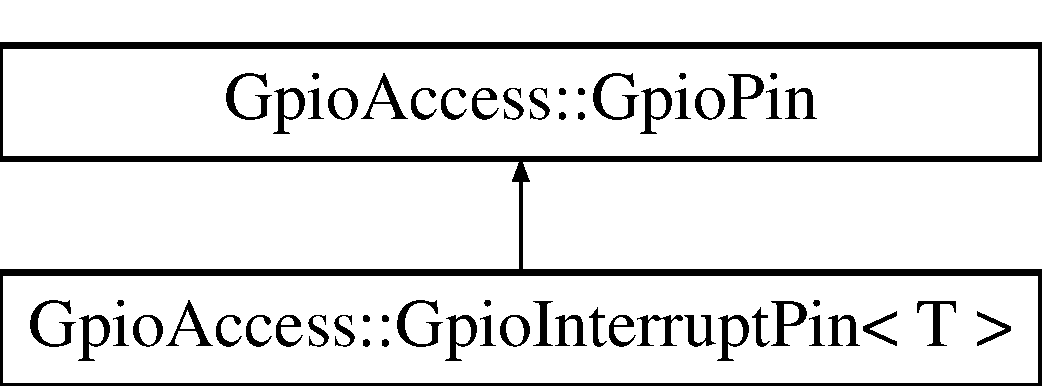
\includegraphics[height=2.000000cm]{class_gpio_access_1_1_gpio_interrupt_pin}
\end{center}
\end{figure}
\subsection*{\-Public \-Member \-Functions}
\begin{DoxyCompactItemize}
\item 
\hyperlink{class_gpio_access_1_1_gpio_interrupt_pin_a73479cbcb8f93e168a8e425d847fab3f}{\-Gpio\-Interrupt\-Pin} (int \hyperlink{class_gpio_access_1_1_gpio_pin_a662d9f6e22d338e0b182b3220a42f25d}{gpio\-Id}, bool pull\-Up=true, bool glitch\-Filter=true, \-T $\ast$object=0, void(\-T\-::$\ast$action)()=0, unsigned int flags=0)
\item 
void \hyperlink{class_gpio_access_1_1_gpio_interrupt_pin_abc83efbda38bea421c0f2ea237fdb240}{activate} ()
\item 
void \hyperlink{class_gpio_access_1_1_gpio_interrupt_pin_aecf2b47b37dc009ee7e01a9c6c5f7f89}{deactivate} ()
\end{DoxyCompactItemize}
\subsection*{\-Static \-Protected \-Member \-Functions}
\begin{DoxyCompactItemize}
\item 
static void \hyperlink{class_gpio_access_1_1_gpio_interrupt_pin_a81df1ecd14f1bb2d0557c89c70f1e3da}{handle\-Signal} (int signum)
\end{DoxyCompactItemize}
\subsection*{\-Protected \-Attributes}
\begin{DoxyCompactItemize}
\item 
int \hyperlink{class_gpio_access_1_1_gpio_interrupt_pin_a1f41ac0250370704c82e2ef827ad55d0}{signal\-Number}
\item 
unsigned int \hyperlink{class_gpio_access_1_1_gpio_interrupt_pin_a60d94e09b68398546d0f8bca1d8f8662}{eint\-Flags}
\end{DoxyCompactItemize}
\subsection*{\-Static \-Protected \-Attributes}
\begin{DoxyCompactItemize}
\item 
static \hyperlink{struct_gpio_access_1_1_signal_action}{\-Signal\-Action}$<$ \-T $>$ \hyperlink{class_gpio_access_1_1_gpio_interrupt_pin_a71835f78bf46796ca311b4357bee2d68}{sig\-Actions} \mbox{[}\-G\-P\-I\-O\-D\-\_\-\-S\-I\-G\-M\-A\-X\mbox{]}
\end{DoxyCompactItemize}


\subsection{\-Detailed \-Description}
\subsubsection*{template$<$class T$>$class Gpio\-Access\-::\-Gpio\-Interrupt\-Pin$<$ T $>$}

\hyperlink{class_gpio_access_1_1_gpio_interrupt_pin}{\-Gpio\-Interrupt\-Pin} es la clase que permite procesar las intrrupciones que se generan en un puerto. 

\-Definition at line 28 of file \-Gpio\-Interrupt\-Pin.\-h.



\subsection{\-Constructor \& \-Destructor \-Documentation}
\hypertarget{class_gpio_access_1_1_gpio_interrupt_pin_a73479cbcb8f93e168a8e425d847fab3f}{\index{\-Gpio\-Access\-::\-Gpio\-Interrupt\-Pin@{\-Gpio\-Access\-::\-Gpio\-Interrupt\-Pin}!\-Gpio\-Interrupt\-Pin@{\-Gpio\-Interrupt\-Pin}}
\index{\-Gpio\-Interrupt\-Pin@{\-Gpio\-Interrupt\-Pin}!GpioAccess::GpioInterruptPin@{\-Gpio\-Access\-::\-Gpio\-Interrupt\-Pin}}
\subsubsection[{\-Gpio\-Interrupt\-Pin}]{\setlength{\rightskip}{0pt plus 5cm}template$<$class T $>$ {\bf \-Gpio\-Access\-::\-Gpio\-Interrupt\-Pin}$<$ \-T $>$\-::{\bf \-Gpio\-Interrupt\-Pin} (
\begin{DoxyParamCaption}
\item[{int}]{gpio\-Id, }
\item[{bool}]{pull\-Up = {\ttfamily true}, }
\item[{bool}]{glitch\-Filter = {\ttfamily true}, }
\item[{\-T $\ast$}]{object = {\ttfamily 0}, }
\item[{void(\-T\-::$\ast$)()}]{action = {\ttfamily 0}, }
\item[{unsigned int}]{flags = {\ttfamily 0}}
\end{DoxyParamCaption}
)}}\label{class_gpio_access_1_1_gpio_interrupt_pin_a73479cbcb8f93e168a8e425d847fab3f}
\-Constructor de \hyperlink{class_gpio_access_1_1_gpio_interrupt_pin}{\-Gpio\-Interrupt\-Pin}. 
\begin{DoxyParams}{\-Parameters}
{\em p\-Gpio\-Id} & es un entero que contiene el identificador del puerto a utilizar. \\
\hline
{\em pull\-Up} & es un valor booleano que define la configuración del resistor pullup. \\
\hline
{\em glitch\-Filter} & es un valor booleano que define la activación del filtro de ruido. \\
\hline
{\em object} & es un puntero a un objeto de tipo \-Tsobre el cual se ejecutará la función action. \\
\hline
{\em action} & es un puntero a una funcion miembro de la clase \-T. \-Es la función que se ejecutará en caso de ocurrir la interrupción externa correspondiente. \\
\hline
{\em flags} & es un entero positivo el cual contiene las banderas de configuración de detección de la interrupción externa. \\
\hline
\end{DoxyParams}

\begin{DoxyExceptions}{\-Exceptions}
{\em runtime\-\_\-error.} & \\
\hline
\end{DoxyExceptions}


\-Definition at line 109 of file \-Gpio\-Interrupt\-Pin.\-h.



\subsection{\-Member \-Function \-Documentation}
\hypertarget{class_gpio_access_1_1_gpio_interrupt_pin_abc83efbda38bea421c0f2ea237fdb240}{\index{\-Gpio\-Access\-::\-Gpio\-Interrupt\-Pin@{\-Gpio\-Access\-::\-Gpio\-Interrupt\-Pin}!activate@{activate}}
\index{activate@{activate}!GpioAccess::GpioInterruptPin@{\-Gpio\-Access\-::\-Gpio\-Interrupt\-Pin}}
\subsubsection[{activate}]{\setlength{\rightskip}{0pt plus 5cm}template$<$class T $>$ void {\bf \-Gpio\-Access\-::\-Gpio\-Interrupt\-Pin}$<$ \-T $>$\-::{\bf activate} (
\begin{DoxyParamCaption}
{}
\end{DoxyParamCaption}
)}}\label{class_gpio_access_1_1_gpio_interrupt_pin_abc83efbda38bea421c0f2ea237fdb240}
\-La función activate activa la deteccón de interrupción. 
\begin{DoxyExceptions}{\-Exceptions}
{\em runtime\-\_\-error.} & \\
\hline
\end{DoxyExceptions}


\-Definition at line 138 of file \-Gpio\-Interrupt\-Pin.\-h.

\hypertarget{class_gpio_access_1_1_gpio_interrupt_pin_aecf2b47b37dc009ee7e01a9c6c5f7f89}{\index{\-Gpio\-Access\-::\-Gpio\-Interrupt\-Pin@{\-Gpio\-Access\-::\-Gpio\-Interrupt\-Pin}!deactivate@{deactivate}}
\index{deactivate@{deactivate}!GpioAccess::GpioInterruptPin@{\-Gpio\-Access\-::\-Gpio\-Interrupt\-Pin}}
\subsubsection[{deactivate}]{\setlength{\rightskip}{0pt plus 5cm}template$<$class T $>$ void {\bf \-Gpio\-Access\-::\-Gpio\-Interrupt\-Pin}$<$ \-T $>$\-::{\bf deactivate} (
\begin{DoxyParamCaption}
{}
\end{DoxyParamCaption}
)}}\label{class_gpio_access_1_1_gpio_interrupt_pin_aecf2b47b37dc009ee7e01a9c6c5f7f89}
\-La función deactivate desactiva la deteccón de interrupción. 
\begin{DoxyExceptions}{\-Exceptions}
{\em runtime\-\_\-error.} & \\
\hline
\end{DoxyExceptions}


\-Definition at line 156 of file \-Gpio\-Interrupt\-Pin.\-h.

\hypertarget{class_gpio_access_1_1_gpio_interrupt_pin_a81df1ecd14f1bb2d0557c89c70f1e3da}{\index{\-Gpio\-Access\-::\-Gpio\-Interrupt\-Pin@{\-Gpio\-Access\-::\-Gpio\-Interrupt\-Pin}!handle\-Signal@{handle\-Signal}}
\index{handle\-Signal@{handle\-Signal}!GpioAccess::GpioInterruptPin@{\-Gpio\-Access\-::\-Gpio\-Interrupt\-Pin}}
\subsubsection[{handle\-Signal}]{\setlength{\rightskip}{0pt plus 5cm}template$<$class T $>$ void {\bf \-Gpio\-Access\-::\-Gpio\-Interrupt\-Pin}$<$ \-T $>$\-::{\bf handle\-Signal} (
\begin{DoxyParamCaption}
\item[{int}]{signum}
\end{DoxyParamCaption}
)\hspace{0.3cm}{\ttfamily  \mbox{[}static, protected\mbox{]}}}}\label{class_gpio_access_1_1_gpio_interrupt_pin_a81df1ecd14f1bb2d0557c89c70f1e3da}
\-La función handle\-Signal será ejecutada de forma estática al recibir las señales del sistema operativo. 
\begin{DoxyParams}{\-Parameters}
{\em signum} & es un entero positivo que contendrá el número de la señal recibida del sistema operativo. \\
\hline
\end{DoxyParams}


\-Definition at line 174 of file \-Gpio\-Interrupt\-Pin.\-h.



\subsection{\-Member \-Data \-Documentation}
\hypertarget{class_gpio_access_1_1_gpio_interrupt_pin_a60d94e09b68398546d0f8bca1d8f8662}{\index{\-Gpio\-Access\-::\-Gpio\-Interrupt\-Pin@{\-Gpio\-Access\-::\-Gpio\-Interrupt\-Pin}!eint\-Flags@{eint\-Flags}}
\index{eint\-Flags@{eint\-Flags}!GpioAccess::GpioInterruptPin@{\-Gpio\-Access\-::\-Gpio\-Interrupt\-Pin}}
\subsubsection[{eint\-Flags}]{\setlength{\rightskip}{0pt plus 5cm}template$<$class T $>$ unsigned int {\bf \-Gpio\-Access\-::\-Gpio\-Interrupt\-Pin}$<$ \-T $>$\-::{\bf eint\-Flags}\hspace{0.3cm}{\ttfamily  \mbox{[}protected\mbox{]}}}}\label{class_gpio_access_1_1_gpio_interrupt_pin_a60d94e09b68398546d0f8bca1d8f8662}
flags es un entero positivo el cual almacena las banderas de configuración de detección de la interrupción externa. 

\-Definition at line 76 of file \-Gpio\-Interrupt\-Pin.\-h.

\hypertarget{class_gpio_access_1_1_gpio_interrupt_pin_a71835f78bf46796ca311b4357bee2d68}{\index{\-Gpio\-Access\-::\-Gpio\-Interrupt\-Pin@{\-Gpio\-Access\-::\-Gpio\-Interrupt\-Pin}!sig\-Actions@{sig\-Actions}}
\index{sig\-Actions@{sig\-Actions}!GpioAccess::GpioInterruptPin@{\-Gpio\-Access\-::\-Gpio\-Interrupt\-Pin}}
\subsubsection[{sig\-Actions}]{\setlength{\rightskip}{0pt plus 5cm}template$<$class T $>$ {\bf \-Gpio\-Access\-::\-Signal\-Action}$<$ \-T $>$ {\bf \-Gpio\-Access\-::\-Gpio\-Interrupt\-Pin}$<$ \-T $>$\-::{\bf sig\-Actions}\hspace{0.3cm}{\ttfamily  \mbox{[}static, protected\mbox{]}}}}\label{class_gpio_access_1_1_gpio_interrupt_pin_a71835f78bf46796ca311b4357bee2d68}
sig\-Actions es un arreglo estático donde se almacena la información necesaria para procesar las señales del resibidas del sistema operativo. 

\-Definition at line 83 of file \-Gpio\-Interrupt\-Pin.\-h.

\hypertarget{class_gpio_access_1_1_gpio_interrupt_pin_a1f41ac0250370704c82e2ef827ad55d0}{\index{\-Gpio\-Access\-::\-Gpio\-Interrupt\-Pin@{\-Gpio\-Access\-::\-Gpio\-Interrupt\-Pin}!signal\-Number@{signal\-Number}}
\index{signal\-Number@{signal\-Number}!GpioAccess::GpioInterruptPin@{\-Gpio\-Access\-::\-Gpio\-Interrupt\-Pin}}
\subsubsection[{signal\-Number}]{\setlength{\rightskip}{0pt plus 5cm}template$<$class T $>$ int {\bf \-Gpio\-Access\-::\-Gpio\-Interrupt\-Pin}$<$ \-T $>$\-::{\bf signal\-Number}\hspace{0.3cm}{\ttfamily  \mbox{[}protected\mbox{]}}}}\label{class_gpio_access_1_1_gpio_interrupt_pin_a1f41ac0250370704c82e2ef827ad55d0}
signal\-Number es un entero positivo que almacena el número de la señal que se recibirá en caso de ocurrir la interrupción correspondiente. 

\-Definition at line 70 of file \-Gpio\-Interrupt\-Pin.\-h.



\-The documentation for this class was generated from the following file\-:\begin{DoxyCompactItemize}
\item 
src/access/\-Gpio\-Interrupt\-Pin.\-h\end{DoxyCompactItemize}

\hypertarget{class_gpio_access_1_1_gpio_output_pin}{\section{\-Gpio\-Access\-:\-:\-Gpio\-Output\-Pin \-Class \-Reference}
\label{class_gpio_access_1_1_gpio_output_pin}\index{\-Gpio\-Access\-::\-Gpio\-Output\-Pin@{\-Gpio\-Access\-::\-Gpio\-Output\-Pin}}
}


{\ttfamily \#include $<$\-Gpio\-Output\-Pin.\-h$>$}

\-Inheritance diagram for \-Gpio\-Access\-:\-:\-Gpio\-Output\-Pin\-:\begin{figure}[H]
\begin{center}
\leavevmode
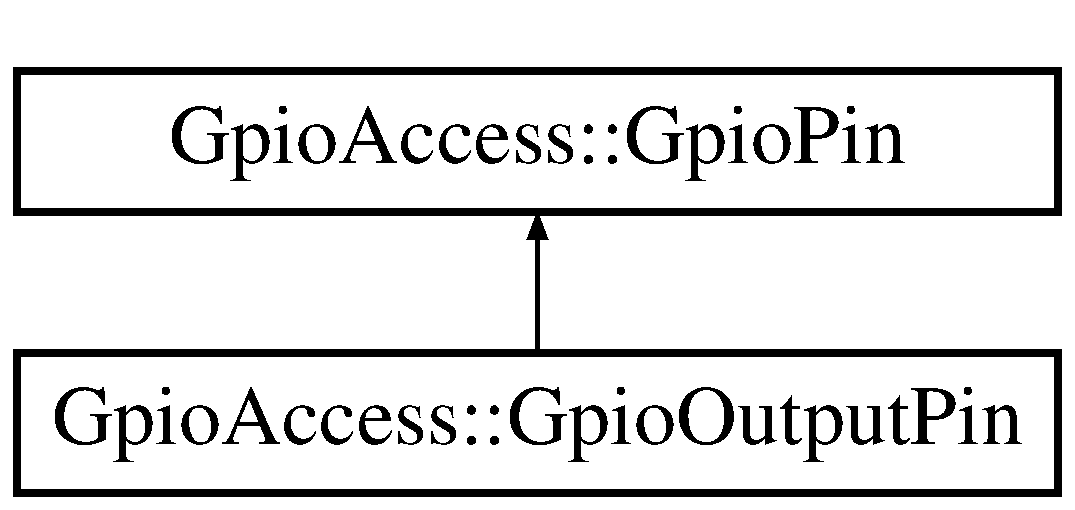
\includegraphics[height=2.000000cm]{class_gpio_access_1_1_gpio_output_pin}
\end{center}
\end{figure}
\subsection*{\-Public \-Member \-Functions}
\begin{DoxyCompactItemize}
\item 
\hyperlink{class_gpio_access_1_1_gpio_output_pin_ada0b9cef6c7e820e0f66f316b344f466}{\-Gpio\-Output\-Pin} (int \hyperlink{class_gpio_access_1_1_gpio_pin_a662d9f6e22d338e0b182b3220a42f25d}{gpio\-Id}=0, bool init\-State=false)
\item 
void \hyperlink{class_gpio_access_1_1_gpio_output_pin_ab85d13a9755482435ef14e969ae89425}{write} (bool state)
\item 
\hypertarget{class_gpio_access_1_1_gpio_output_pin_a69bf2e674146c797283ae78df2d7ff04}{void {\bfseries operator=} (bool state)}\label{class_gpio_access_1_1_gpio_output_pin_a69bf2e674146c797283ae78df2d7ff04}

\end{DoxyCompactItemize}


\subsection{\-Detailed \-Description}
\hyperlink{class_gpio_access_1_1_gpio_input_pin}{\-Gpio\-Input\-Pin} es la clase que define las funcionalidades de un puerto de salida. 

\-Definition at line 16 of file \-Gpio\-Output\-Pin.\-h.



\subsection{\-Constructor \& \-Destructor \-Documentation}
\hypertarget{class_gpio_access_1_1_gpio_output_pin_ada0b9cef6c7e820e0f66f316b344f466}{\index{\-Gpio\-Access\-::\-Gpio\-Output\-Pin@{\-Gpio\-Access\-::\-Gpio\-Output\-Pin}!\-Gpio\-Output\-Pin@{\-Gpio\-Output\-Pin}}
\index{\-Gpio\-Output\-Pin@{\-Gpio\-Output\-Pin}!GpioAccess::GpioOutputPin@{\-Gpio\-Access\-::\-Gpio\-Output\-Pin}}
\subsubsection[{\-Gpio\-Output\-Pin}]{\setlength{\rightskip}{0pt plus 5cm}{\bf \-Gpio\-Access\-::\-Gpio\-Output\-Pin\-::\-Gpio\-Output\-Pin} (
\begin{DoxyParamCaption}
\item[{int}]{gpio\-Id = {\ttfamily 0}, }
\item[{bool}]{init\-State = {\ttfamily false}}
\end{DoxyParamCaption}
)}}\label{class_gpio_access_1_1_gpio_output_pin_ada0b9cef6c7e820e0f66f316b344f466}
\-Constructor de \hyperlink{class_gpio_access_1_1_gpio_output_pin}{\-Gpio\-Output\-Pin}. 
\begin{DoxyParams}{\-Parameters}
{\em p\-Gpio\-Id} & es un entero que contiene el identificador del puerto a utilizar. \\
\hline
{\em init\-State} & es un valor booleano que define el estado inicial del puerto de salida. \\
\hline
\end{DoxyParams}

\begin{DoxyExceptions}{\-Exceptions}
{\em runtime\-\_\-error.} & \\
\hline
\end{DoxyExceptions}


\-Definition at line 12 of file \-Gpio\-Output\-Pin.\-cpp.



\subsection{\-Member \-Function \-Documentation}
\hypertarget{class_gpio_access_1_1_gpio_output_pin_ab85d13a9755482435ef14e969ae89425}{\index{\-Gpio\-Access\-::\-Gpio\-Output\-Pin@{\-Gpio\-Access\-::\-Gpio\-Output\-Pin}!write@{write}}
\index{write@{write}!GpioAccess::GpioOutputPin@{\-Gpio\-Access\-::\-Gpio\-Output\-Pin}}
\subsubsection[{write}]{\setlength{\rightskip}{0pt plus 5cm}void {\bf \-Gpio\-Access\-::\-Gpio\-Output\-Pin\-::write} (
\begin{DoxyParamCaption}
\item[{bool}]{state}
\end{DoxyParamCaption}
)}}\label{class_gpio_access_1_1_gpio_output_pin_ab85d13a9755482435ef14e969ae89425}
\-La función write establece el estado del puerto de salida. 
\begin{DoxyParams}{\-Parameters}
{\em state} & es un valor booleano el cual se establecerá como salida del puerto. \\
\hline
\end{DoxyParams}

\begin{DoxyExceptions}{\-Exceptions}
{\em runtime\-\_\-error.} & \\
\hline
\end{DoxyExceptions}


\-Definition at line 21 of file \-Gpio\-Output\-Pin.\-cpp.



\-The documentation for this class was generated from the following files\-:\begin{DoxyCompactItemize}
\item 
src/access/\-Gpio\-Output\-Pin.\-h\item 
src/access/\-Gpio\-Output\-Pin.\-cpp\end{DoxyCompactItemize}

\hypertarget{class_gpio_access_1_1_gpio_output_port}{\section{\-Gpio\-Access\-:\-:\-Gpio\-Output\-Port \-Class \-Reference}
\label{class_gpio_access_1_1_gpio_output_port}\index{\-Gpio\-Access\-::\-Gpio\-Output\-Port@{\-Gpio\-Access\-::\-Gpio\-Output\-Port}}
}


{\ttfamily \#include $<$\-Gpio\-Output\-Port.\-h$>$}

\-Inheritance diagram for \-Gpio\-Access\-:\-:\-Gpio\-Output\-Port\-:\begin{figure}[H]
\begin{center}
\leavevmode
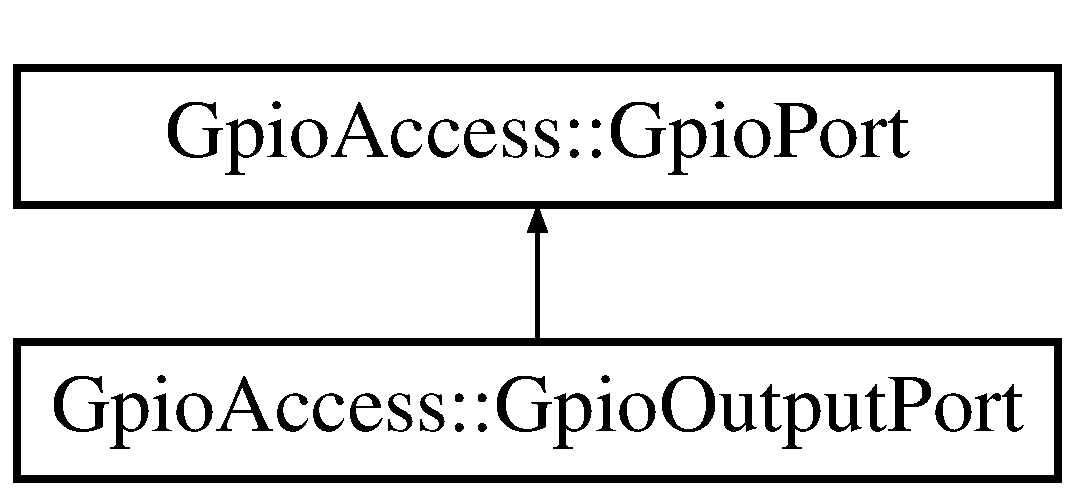
\includegraphics[height=2.000000cm]{class_gpio_access_1_1_gpio_output_port}
\end{center}
\end{figure}
\subsection*{\-Public \-Member \-Functions}
\begin{DoxyCompactItemize}
\item 
\hyperlink{class_gpio_access_1_1_gpio_output_port_aad40d2242724e4b4a4ce664748b8232d}{\-Gpio\-Output\-Port} (int $\ast$bits\-Ids, int \hyperlink{class_gpio_access_1_1_gpio_port_a7708b465b3c98a32e592ee985c3dcf8b}{bit\-Count}, unsigned int init\-State=0)
\item 
void \hyperlink{class_gpio_access_1_1_gpio_output_port_abc3c17790a4a89df9dd73e0818dade4a}{write} (unsigned int state)
\item 
\hypertarget{class_gpio_access_1_1_gpio_output_port_a073ac74b839c691244f4c7575ed88344}{\hyperlink{class_gpio_access_1_1_gpio_output_pin}{\-Gpio\-Access\-::\-Gpio\-Output\-Pin} {\bfseries operator\mbox{[}$\,$\mbox{]}} (unsigned int pos)}\label{class_gpio_access_1_1_gpio_output_port_a073ac74b839c691244f4c7575ed88344}

\end{DoxyCompactItemize}
\subsection*{\-Protected \-Attributes}
\begin{DoxyCompactItemize}
\item 
\hyperlink{class_gpio_access_1_1_gpio_output_pin}{\-Gpio\-Access\-::\-Gpio\-Output\-Pin} $\ast$ \hyperlink{class_gpio_access_1_1_gpio_output_port_a490b121699442f0a08beef308a867f1b}{output\-Bits}
\end{DoxyCompactItemize}


\subsection{\-Detailed \-Description}
\hyperlink{class_gpio_access_1_1_gpio_input_port}{\-Gpio\-Input\-Port} es la clase que define las funcionalidades de un bus de salida. 

\-Definition at line 21 of file \-Gpio\-Output\-Port.\-h.



\subsection{\-Constructor \& \-Destructor \-Documentation}
\hypertarget{class_gpio_access_1_1_gpio_output_port_aad40d2242724e4b4a4ce664748b8232d}{\index{\-Gpio\-Access\-::\-Gpio\-Output\-Port@{\-Gpio\-Access\-::\-Gpio\-Output\-Port}!\-Gpio\-Output\-Port@{\-Gpio\-Output\-Port}}
\index{\-Gpio\-Output\-Port@{\-Gpio\-Output\-Port}!GpioAccess::GpioOutputPort@{\-Gpio\-Access\-::\-Gpio\-Output\-Port}}
\subsubsection[{\-Gpio\-Output\-Port}]{\setlength{\rightskip}{0pt plus 5cm}{\bf \-Gpio\-Access\-::\-Gpio\-Output\-Port\-::\-Gpio\-Output\-Port} (
\begin{DoxyParamCaption}
\item[{int $\ast$}]{bits\-Ids, }
\item[{int}]{bit\-Count, }
\item[{unsigned int}]{init\-State = {\ttfamily 0}}
\end{DoxyParamCaption}
)}}\label{class_gpio_access_1_1_gpio_output_port_aad40d2242724e4b4a4ce664748b8232d}
\-Constructor de \hyperlink{class_gpio_access_1_1_gpio_output_port}{\-Gpio\-Output\-Port}. 
\begin{DoxyParams}{\-Parameters}
{\em bits\-Ids} & es un arreglo de enteros los cuales corresponden con los identificadores de los puertos que conforman el bus de salida. \\
\hline
{\em p\-Bit\-Count} & cantidad de bits del bus de salida. \\
\hline
{\em init\-State} & es un entero positivo que define el estado inicial del bus de salida. \\
\hline
\end{DoxyParams}

\begin{DoxyExceptions}{\-Exceptions}
{\em runtime\-\_\-error.} & \\
\hline
\end{DoxyExceptions}


\-Definition at line 8 of file \-Gpio\-Output\-Port.\-cpp.



\subsection{\-Member \-Function \-Documentation}
\hypertarget{class_gpio_access_1_1_gpio_output_port_abc3c17790a4a89df9dd73e0818dade4a}{\index{\-Gpio\-Access\-::\-Gpio\-Output\-Port@{\-Gpio\-Access\-::\-Gpio\-Output\-Port}!write@{write}}
\index{write@{write}!GpioAccess::GpioOutputPort@{\-Gpio\-Access\-::\-Gpio\-Output\-Port}}
\subsubsection[{write}]{\setlength{\rightskip}{0pt plus 5cm}void {\bf \-Gpio\-Access\-::\-Gpio\-Output\-Port\-::write} (
\begin{DoxyParamCaption}
\item[{unsigned int}]{state}
\end{DoxyParamCaption}
)}}\label{class_gpio_access_1_1_gpio_output_port_abc3c17790a4a89df9dd73e0818dade4a}
\-La función write establece el estado del bus de salida. 
\begin{DoxyParams}{\-Parameters}
{\em state} & es un entero positivo el cual se establecerá como salida del bus. \\
\hline
\end{DoxyParams}

\begin{DoxyExceptions}{\-Exceptions}
{\em runtime\-\_\-error.} & \\
\hline
\end{DoxyExceptions}


\-Definition at line 27 of file \-Gpio\-Output\-Port.\-cpp.



\subsection{\-Member \-Data \-Documentation}
\hypertarget{class_gpio_access_1_1_gpio_output_port_a490b121699442f0a08beef308a867f1b}{\index{\-Gpio\-Access\-::\-Gpio\-Output\-Port@{\-Gpio\-Access\-::\-Gpio\-Output\-Port}!output\-Bits@{output\-Bits}}
\index{output\-Bits@{output\-Bits}!GpioAccess::GpioOutputPort@{\-Gpio\-Access\-::\-Gpio\-Output\-Port}}
\subsubsection[{output\-Bits}]{\setlength{\rightskip}{0pt plus 5cm}{\bf \-Gpio\-Access\-::\-Gpio\-Output\-Pin}$\ast$ {\bf \-Gpio\-Access\-::\-Gpio\-Output\-Port\-::output\-Bits}\hspace{0.3cm}{\ttfamily  \mbox{[}protected\mbox{]}}}}\label{class_gpio_access_1_1_gpio_output_port_a490b121699442f0a08beef308a867f1b}
output\-Bits es un arreglo \hyperlink{class_gpio_access_1_1_gpio_output_port}{\-Gpio\-Output\-Port} que almacena los puertos de salida que conforman el bus. 

\-Definition at line 52 of file \-Gpio\-Output\-Port.\-h.



\-The documentation for this class was generated from the following files\-:\begin{DoxyCompactItemize}
\item 
src/access/\-Gpio\-Output\-Port.\-h\item 
src/access/\-Gpio\-Output\-Port.\-cpp\end{DoxyCompactItemize}

\hypertarget{class_gpio_access_1_1_gpio_pin}{\section{\-Gpio\-Access\-:\-:\-Gpio\-Pin \-Class \-Reference}
\label{class_gpio_access_1_1_gpio_pin}\index{\-Gpio\-Access\-::\-Gpio\-Pin@{\-Gpio\-Access\-::\-Gpio\-Pin}}
}


{\ttfamily \#include $<$\-Gpio\-Pin.\-h$>$}

\-Inheritance diagram for \-Gpio\-Access\-:\-:\-Gpio\-Pin\-:\begin{figure}[H]
\begin{center}
\leavevmode
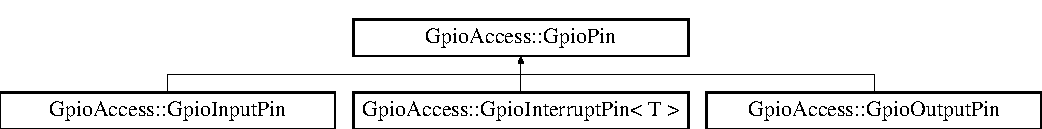
\includegraphics[height=1.728395cm]{class_gpio_access_1_1_gpio_pin}
\end{center}
\end{figure}
\subsection*{\-Public \-Member \-Functions}
\begin{DoxyCompactItemize}
\item 
\hyperlink{class_gpio_access_1_1_gpio_pin_ad212b4623cd8e4f6dda1335774f54f2f}{\-Gpio\-Pin} (int p\-Gpio\-Id)
\item 
bool \hyperlink{class_gpio_access_1_1_gpio_pin_a91c4e6b319184b943ed6094d10056348}{read} ()
\end{DoxyCompactItemize}
\subsection*{\-Protected \-Member \-Functions}
\begin{DoxyCompactItemize}
\item 
int \hyperlink{class_gpio_access_1_1_gpio_pin_a407236169f0e60364db7618c12fe29e9}{ioctl\-Cmd} (unsigned int cmd, unsigned int value=0)
\end{DoxyCompactItemize}
\subsection*{\-Protected \-Attributes}
\begin{DoxyCompactItemize}
\item 
int \hyperlink{class_gpio_access_1_1_gpio_pin_a662d9f6e22d338e0b182b3220a42f25d}{gpio\-Id}
\end{DoxyCompactItemize}
\subsection*{\-Static \-Protected \-Attributes}
\begin{DoxyCompactItemize}
\item 
static int \hyperlink{class_gpio_access_1_1_gpio_pin_aa3cfd18199fbe18a6d7d74a7a753dbab}{file} = 0
\end{DoxyCompactItemize}


\subsection{\-Detailed \-Description}
\hyperlink{class_gpio_access_1_1_gpio_pin}{\-Gpio\-Pin} es la clase base para los puertos \-G\-P\-I\-O 

\-Definition at line 13 of file \-Gpio\-Pin.\-h.



\subsection{\-Constructor \& \-Destructor \-Documentation}
\hypertarget{class_gpio_access_1_1_gpio_pin_ad212b4623cd8e4f6dda1335774f54f2f}{\index{\-Gpio\-Access\-::\-Gpio\-Pin@{\-Gpio\-Access\-::\-Gpio\-Pin}!\-Gpio\-Pin@{\-Gpio\-Pin}}
\index{\-Gpio\-Pin@{\-Gpio\-Pin}!GpioAccess::GpioPin@{\-Gpio\-Access\-::\-Gpio\-Pin}}
\subsubsection[{\-Gpio\-Pin}]{\setlength{\rightskip}{0pt plus 5cm}{\bf \-Gpio\-Access\-::\-Gpio\-Pin\-::\-Gpio\-Pin} (
\begin{DoxyParamCaption}
\item[{int}]{p\-Gpio\-Id}
\end{DoxyParamCaption}
)}}\label{class_gpio_access_1_1_gpio_pin_ad212b4623cd8e4f6dda1335774f54f2f}
\-Constructor de \hyperlink{class_gpio_access_1_1_gpio_pin}{\-Gpio\-Pin}. 
\begin{DoxyParams}{\-Parameters}
{\em p\-Gpio\-Id} & es un entero que contiene el identificador del puerto a utilizar. \\
\hline
\end{DoxyParams}

\begin{DoxyExceptions}{\-Exceptions}
{\em runtime\-\_\-error.} & \\
\hline
\end{DoxyExceptions}


\-Definition at line 13 of file \-Gpio\-Pin.\-cpp.



\subsection{\-Member \-Function \-Documentation}
\hypertarget{class_gpio_access_1_1_gpio_pin_a407236169f0e60364db7618c12fe29e9}{\index{\-Gpio\-Access\-::\-Gpio\-Pin@{\-Gpio\-Access\-::\-Gpio\-Pin}!ioctl\-Cmd@{ioctl\-Cmd}}
\index{ioctl\-Cmd@{ioctl\-Cmd}!GpioAccess::GpioPin@{\-Gpio\-Access\-::\-Gpio\-Pin}}
\subsubsection[{ioctl\-Cmd}]{\setlength{\rightskip}{0pt plus 5cm}int {\bf \-Gpio\-Access\-::\-Gpio\-Pin\-::ioctl\-Cmd} (
\begin{DoxyParamCaption}
\item[{unsigned int}]{cmd, }
\item[{unsigned int}]{value = {\ttfamily 0}}
\end{DoxyParamCaption}
)\hspace{0.3cm}{\ttfamily  \mbox{[}protected\mbox{]}}}}\label{class_gpio_access_1_1_gpio_pin_a407236169f0e60364db7618c12fe29e9}
\-La función ioctl\-Cmd es la encargada de hacer el llamado ioctl al driver. 
\begin{DoxyParams}{\-Parameters}
{\em cmd} & es un valor entero positivo que corresponde el comando a ejecutar. \\
\hline
{\em value} & es un valor entero positivo el cual va a utilizar el comando si es necesario. \\
\hline
\end{DoxyParams}
\begin{DoxyReturn}{\-Returns}
\-Devuelve el valor entero retornado por la ejecución del comando ioctl cmd. 
\end{DoxyReturn}


\-Definition at line 23 of file \-Gpio\-Pin.\-cpp.

\hypertarget{class_gpio_access_1_1_gpio_pin_a91c4e6b319184b943ed6094d10056348}{\index{\-Gpio\-Access\-::\-Gpio\-Pin@{\-Gpio\-Access\-::\-Gpio\-Pin}!read@{read}}
\index{read@{read}!GpioAccess::GpioPin@{\-Gpio\-Access\-::\-Gpio\-Pin}}
\subsubsection[{read}]{\setlength{\rightskip}{0pt plus 5cm}bool {\bf \-Gpio\-Access\-::\-Gpio\-Pin\-::read} (
\begin{DoxyParamCaption}
{}
\end{DoxyParamCaption}
)}}\label{class_gpio_access_1_1_gpio_pin_a91c4e6b319184b943ed6094d10056348}
\-La función read lee el valor presente en un puerto. \begin{DoxyReturn}{\-Returns}
\-Devuelve un valor booleano positivo correspondiente a la lectura del bus de entrada. 
\end{DoxyReturn}

\begin{DoxyExceptions}{\-Exceptions}
{\em runtime\-\_\-error.} & \\
\hline
\end{DoxyExceptions}


\-Definition at line 31 of file \-Gpio\-Pin.\-cpp.



\subsection{\-Member \-Data \-Documentation}
\hypertarget{class_gpio_access_1_1_gpio_pin_aa3cfd18199fbe18a6d7d74a7a753dbab}{\index{\-Gpio\-Access\-::\-Gpio\-Pin@{\-Gpio\-Access\-::\-Gpio\-Pin}!file@{file}}
\index{file@{file}!GpioAccess::GpioPin@{\-Gpio\-Access\-::\-Gpio\-Pin}}
\subsubsection[{file}]{\setlength{\rightskip}{0pt plus 5cm}int {\bf \-Gpio\-Access\-::\-Gpio\-Pin\-::file} = 0\hspace{0.3cm}{\ttfamily  \mbox{[}static, protected\mbox{]}}}}\label{class_gpio_access_1_1_gpio_pin_aa3cfd18199fbe18a6d7d74a7a753dbab}
file es un entero que elmacena del descriptor del fichero de acceso al driver gpio (en linux /dev/gpio2440). 

\-Definition at line 54 of file \-Gpio\-Pin.\-h.

\hypertarget{class_gpio_access_1_1_gpio_pin_a662d9f6e22d338e0b182b3220a42f25d}{\index{\-Gpio\-Access\-::\-Gpio\-Pin@{\-Gpio\-Access\-::\-Gpio\-Pin}!gpio\-Id@{gpio\-Id}}
\index{gpio\-Id@{gpio\-Id}!GpioAccess::GpioPin@{\-Gpio\-Access\-::\-Gpio\-Pin}}
\subsubsection[{gpio\-Id}]{\setlength{\rightskip}{0pt plus 5cm}int {\bf \-Gpio\-Access\-::\-Gpio\-Pin\-::gpio\-Id}\hspace{0.3cm}{\ttfamily  \mbox{[}protected\mbox{]}}}}\label{class_gpio_access_1_1_gpio_pin_a662d9f6e22d338e0b182b3220a42f25d}
gpio\-Id es un entero que contiene el identificador del puerto. 

\-Definition at line 48 of file \-Gpio\-Pin.\-h.



\-The documentation for this class was generated from the following files\-:\begin{DoxyCompactItemize}
\item 
src/access/\-Gpio\-Pin.\-h\item 
src/access/\-Gpio\-Pin.\-cpp\end{DoxyCompactItemize}

\hypertarget{class_gpio_access_1_1_gpio_port}{\section{\-Gpio\-Access\-:\-:\-Gpio\-Port \-Class \-Reference}
\label{class_gpio_access_1_1_gpio_port}\index{\-Gpio\-Access\-::\-Gpio\-Port@{\-Gpio\-Access\-::\-Gpio\-Port}}
}


{\ttfamily \#include $<$\-Gpio\-Port.\-h$>$}

\-Inheritance diagram for \-Gpio\-Access\-:\-:\-Gpio\-Port\-:\begin{figure}[H]
\begin{center}
\leavevmode
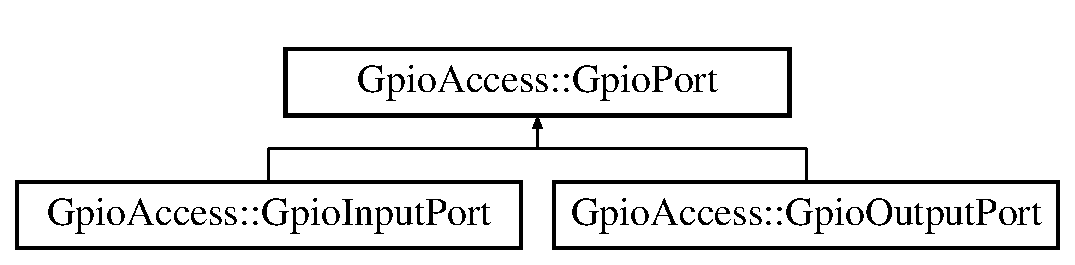
\includegraphics[height=2.000000cm]{class_gpio_access_1_1_gpio_port}
\end{center}
\end{figure}
\subsection*{\-Public \-Member \-Functions}
\begin{DoxyCompactItemize}
\item 
\hyperlink{class_gpio_access_1_1_gpio_port_aed72a6006ccc890557f66297d67b43cc}{\-Gpio\-Port} (unsigned int \hyperlink{class_gpio_access_1_1_gpio_port_a7708b465b3c98a32e592ee985c3dcf8b}{bit\-Count})
\end{DoxyCompactItemize}
\subsection*{\-Protected \-Attributes}
\begin{DoxyCompactItemize}
\item 
unsigned int \hyperlink{class_gpio_access_1_1_gpio_port_a7708b465b3c98a32e592ee985c3dcf8b}{bit\-Count}
\end{DoxyCompactItemize}


\subsection{\-Detailed \-Description}
\hyperlink{class_gpio_access_1_1_gpio_port}{\-Gpio\-Port} es la clase base para los bus de datos de entrada y salida. 

\-Definition at line 16 of file \-Gpio\-Port.\-h.



\subsection{\-Constructor \& \-Destructor \-Documentation}
\hypertarget{class_gpio_access_1_1_gpio_port_aed72a6006ccc890557f66297d67b43cc}{\index{\-Gpio\-Access\-::\-Gpio\-Port@{\-Gpio\-Access\-::\-Gpio\-Port}!\-Gpio\-Port@{\-Gpio\-Port}}
\index{\-Gpio\-Port@{\-Gpio\-Port}!GpioAccess::GpioPort@{\-Gpio\-Access\-::\-Gpio\-Port}}
\subsubsection[{\-Gpio\-Port}]{\setlength{\rightskip}{0pt plus 5cm}{\bf \-Gpio\-Access\-::\-Gpio\-Port\-::\-Gpio\-Port} (
\begin{DoxyParamCaption}
\item[{unsigned int}]{bit\-Count}
\end{DoxyParamCaption}
)}}\label{class_gpio_access_1_1_gpio_port_aed72a6006ccc890557f66297d67b43cc}
\-Constructor de \hyperlink{class_gpio_access_1_1_gpio_port}{\-Gpio\-Port}. 
\begin{DoxyParams}{\-Parameters}
{\em p\-Bit\-Count} & es la cantidad de bits del bus datos. \\
\hline
\end{DoxyParams}

\begin{DoxyExceptions}{\-Exceptions}
{\em runtime\-\_\-error.} & \\
\hline
\end{DoxyExceptions}


\-Definition at line 7 of file \-Gpio\-Port.\-cpp.



\subsection{\-Member \-Data \-Documentation}
\hypertarget{class_gpio_access_1_1_gpio_port_a7708b465b3c98a32e592ee985c3dcf8b}{\index{\-Gpio\-Access\-::\-Gpio\-Port@{\-Gpio\-Access\-::\-Gpio\-Port}!bit\-Count@{bit\-Count}}
\index{bit\-Count@{bit\-Count}!GpioAccess::GpioPort@{\-Gpio\-Access\-::\-Gpio\-Port}}
\subsubsection[{bit\-Count}]{\setlength{\rightskip}{0pt plus 5cm}unsigned int {\bf \-Gpio\-Access\-::\-Gpio\-Port\-::bit\-Count}\hspace{0.3cm}{\ttfamily  \mbox{[}protected\mbox{]}}}}\label{class_gpio_access_1_1_gpio_port_a7708b465b3c98a32e592ee985c3dcf8b}
bit\-Count almacena la cantidad de bits del bus de datos. 

\-Definition at line 30 of file \-Gpio\-Port.\-h.



\-The documentation for this class was generated from the following files\-:\begin{DoxyCompactItemize}
\item 
src/access/\-Gpio\-Port.\-h\item 
src/access/\-Gpio\-Port.\-cpp\end{DoxyCompactItemize}

\hypertarget{struct_gpio_access_1_1_signal_action}{\section{\-Gpio\-Access\-:\-:\-Signal\-Action$<$ \-T $>$ \-Struct \-Template \-Reference}
\label{struct_gpio_access_1_1_signal_action}\index{\-Gpio\-Access\-::\-Signal\-Action$<$ T $>$@{\-Gpio\-Access\-::\-Signal\-Action$<$ T $>$}}
}


{\ttfamily \#include $<$\-Gpio\-Interrupt\-Pin.\-h$>$}

\subsection*{\-Public \-Attributes}
\begin{DoxyCompactItemize}
\item 
\hypertarget{struct_gpio_access_1_1_signal_action_a42d425871977d70e31aa85a218a4e251}{\-T $\ast$ {\bfseries object}}\label{struct_gpio_access_1_1_signal_action_a42d425871977d70e31aa85a218a4e251}

\item 
\hypertarget{struct_gpio_access_1_1_signal_action_a75a653242029a13e2929865c488ed07c}{void(\-T\-::$\ast$ {\bfseries function} )()}\label{struct_gpio_access_1_1_signal_action_a75a653242029a13e2929865c488ed07c}

\end{DoxyCompactItemize}


\subsection{\-Detailed \-Description}
\subsubsection*{template$<$class T$>$struct Gpio\-Access\-::\-Signal\-Action$<$ T $>$}

\hyperlink{struct_gpio_access_1_1_signal_action}{\-Signal\-Action} es una estructura donde se almacena un puntero a objeto de tipo \-T y un puntero a una funcion miembro de la misma clase del objeto. 

\-Definition at line 18 of file \-Gpio\-Interrupt\-Pin.\-h.



\-The documentation for this struct was generated from the following file\-:\begin{DoxyCompactItemize}
\item 
src/access/\-Gpio\-Interrupt\-Pin.\-h\end{DoxyCompactItemize}

\hypertarget{class_test_class}{\section{\-Test\-Class \-Class \-Reference}
\label{class_test_class}\index{\-Test\-Class@{\-Test\-Class}}
}
\subsection*{\-Public \-Member \-Functions}
\begin{DoxyCompactItemize}
\item 
\hypertarget{class_test_class_ab7a8a902ef8358575c0143e0bc27dbcf}{void {\bfseries action} ()}\label{class_test_class_ab7a8a902ef8358575c0143e0bc27dbcf}

\end{DoxyCompactItemize}


\subsection{\-Detailed \-Description}


\-Definition at line 16 of file main.\-cpp.



\-The documentation for this class was generated from the following file\-:\begin{DoxyCompactItemize}
\item 
src/test/main.\-cpp\end{DoxyCompactItemize}

\printindex
\end{document}
